\section{Auswertung}
\label{sec:Auswertung}

\subsection{Umrechnung der Messdaten} % (fold)
\label{sec:umrechnung}
Die im Appendix vorliegenden Diagramme lassen zu, Messdaten mit hoher Genauigkeit in ihren Koordinaten zu bestimmen.
Die x-Koordinaten der auszuwertenden Punkte werden in Bezug auf den eingezeichneten Koordinatenursprung bestimmt und für die Auswertung anhand der Gleichung 
\begin{equation}
	U=a_\text{lin}\cdot x+b_\text{lin}
	\label{eq:umrechnung}
\end{equation}
in eine Spannung $U$ umgerechnet.
Die Einheiten von $a_\text{lin}$ und $b_\text{lin}$ sind gemäß der Größenumrechnung passend gewählt, 
es gelten $[a_\text{lin}]=\si{\volt\per\centi\meter}$ und $[b_\text{lin}]=\si{\volt}$.
Diese fehlerbehaftete Umrechnungsparameter stammen von einer linearen Regression mehrer fester Skalenpunkte, für welche die Spannung bekannt ist.

\begin{table}
	\centering
	\sisetup{table-format = -1.3(1)}
		\begin{tabular}{l S S}
		\toprule
		{Plot Nr.}&\multicolumn{2}{c}{Umrechnungsparameter}\\
		&{$a_\text{lin}$/$\:(\si{\volt\per\centi\meter})$} & {$b_\text{lin}$/$\:\si{\volt}$}\\
		\midrule
		1&		0.403(4)& 	-0.12(6)\\
		2&		0.405(4)& 	0.015(6)\\
		3&		2.89(2)& 	-3.9(2)	\\
		4& 		2.40(3)& 	-1.1(5)	\\
		\end{tabular}
	\caption{Parameter der linearen Regression der Diagramm-Skalen für die Umrechnung der Messdaten; 
	Umrechnung Diagrammlänge zu Spannung.}
	\label{tab:umrechnung}
\end{table}

Analoge Umrechnung ist für die y-Koordinaten in Stromstärken möglich.
\begin{equation}
	I=a'_\text{lin}\cdot x+b'_\text{lin}
	\label{eq:umrechnung}
\end{equation}
Es gelten $[a'_\text{lin}]=\si{\nano\ampere\per\centi\meter}$ und $[b'_\text{lin}]=\si{\nano\ampere}$.


\begin{table}
	\centering
	\sisetup{table-format=1.3}
		\begin{tabular}{l S[table-format=1.3] S[table-format=1.3]}
		\toprule
		{Plot Nr.}&\multicolumn{2}{c}{Umrechnungsparameter}\\
		&{$a'_\text{lin}$/$\:(\si{\nano\ampere\per\centi\meter})$} & {$b'_\text{lin}$/$\:\si{\nano\ampere}$}\\
		\midrule
		1&	0.41& 1.00\\
		2&	1.77& 2.20\\
		\end{tabular}
	\caption{Parameter der linearen Regression der Diagramm-Skalen für die Umrechnung der Messdaten; 
	Umrechnung Diagrammlänge zu Stromstärke.}
	\label{tab:umrechnung}
\end{table}
%Ekalt0.41051.0000
%Ewarm1.77422.2000

% section umrechnung (end)
\subsection{Energieverteilung der Elektronen} % (fold)
\label{sec:energiespektren}
Die im Appendix beigefügten Diagramme \emph{A1} und \emph{A2} werden ausgelesen;
das Millimeterpapier lässt eine Genauigkeit von $\SI{1}{\milli\meter}$ zu.
Die Schrittweite entlang der Abzissenachse wird im Allgemeinen so gewählt, dass einerseits \SI{1}{\centi\meter} nicht überschritten wird und 
andererseits ein Unterschied der Werte entlang der Ordinaten-Achse von mindestens $\SI{1}{\milli\meter}$, die größtmögliche Auflösung beim verwandten Papier, gewährleistet ist.
An Stellen mit linearem Verlauf in guter Näherung ist die Schrittweite groß; 
analog ist sie an Stellen starker Steigungsänderung kleinstmöglich gewählt.
Die eingelesenen Daten sind in Tabellen \ref{tab:E_vert_kalt} und \ref{tab:E_vert_warm} aufgetragen, ihre Darstellung ist in Diagramm \ref{fig:E_vert_kalt} und \ref{fig:E_vert_warm} sichtbar.
\begin{figure}[p]
	\centering
	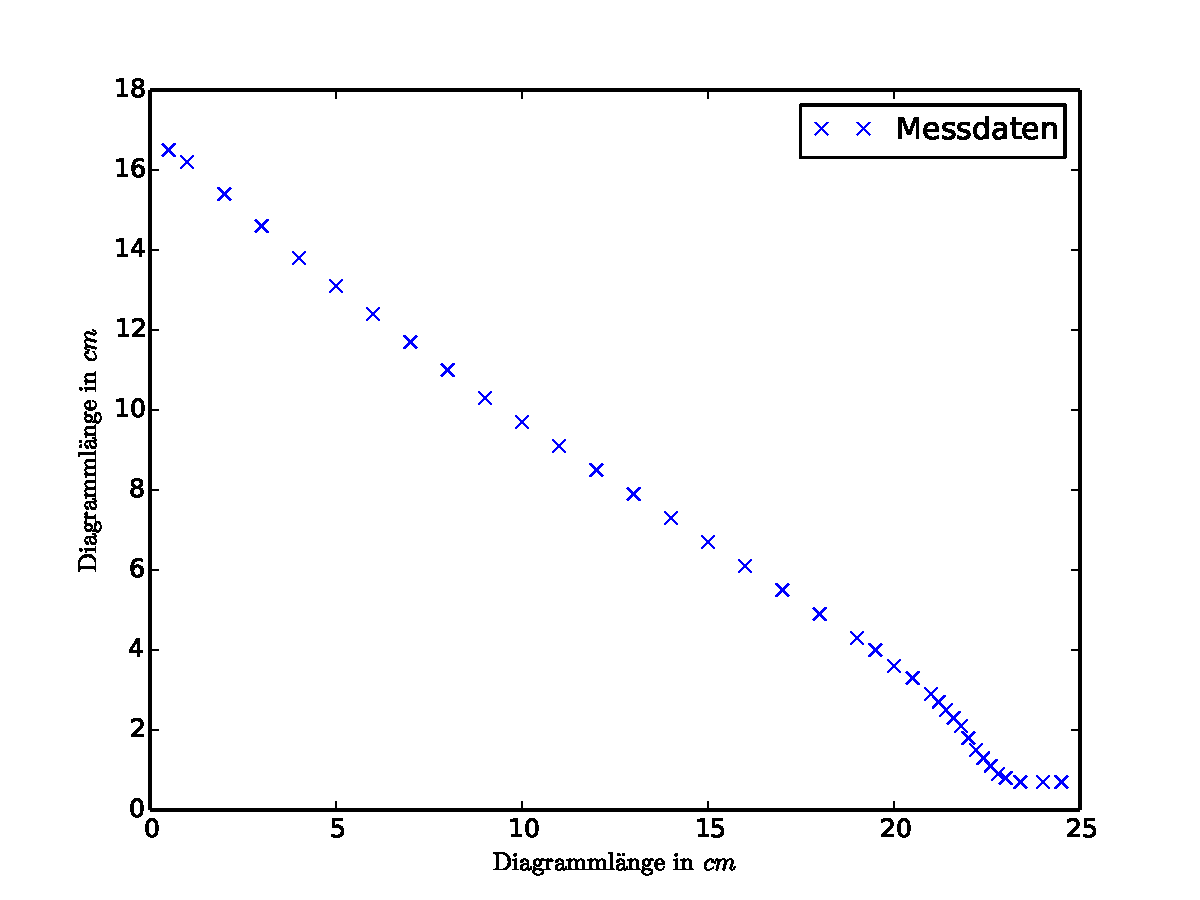
\includegraphics[width=0.7\textwidth]{Bilder/Vert_kalt.pdf}
	\caption{Auftrag der aus Diagramm \emph{A1} entnommenen Daten zum Vergleichen.}
	\label{fig:E_vert_kalt}
\end{figure}
\begin{figure}[p]
	\centering
	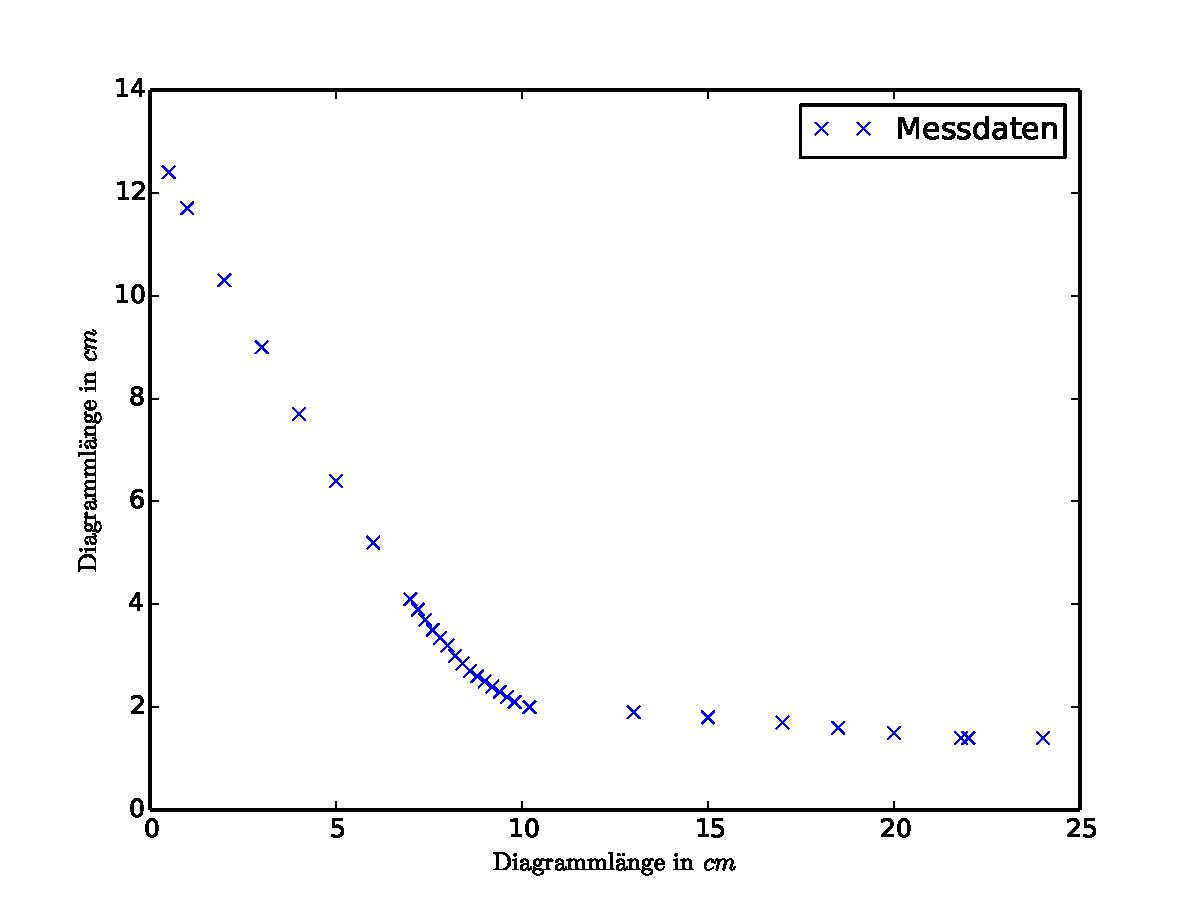
\includegraphics[width=0.7\textwidth]{Bilder/Vert_warm.pdf}
	\caption{Auftrag der aus Diagramm \emph{A2} entnommenen Daten zum Vergleichen.}
	\label{fig:E_vert_warm}
\end{figure}
Die aufgenommene integrale Energieverteilung wird in eine differentielle Energieverteilung umgeformt.
Hierzu wird der Abstand zwischen zwei y-Koordinaten durch den Abstand der dazugehörigen x-Koordinaten geteilt und diese Steigung in der Diagramm \ref{fig:E_vert_kalt}, respektive \ref{fig:E_vert_warm}, aufgetragen. 
Diese Steigung wird in die Mitte zwischen den beiden x-Koordinaten gesetzt, damit entspricht das Verfahren einer angenährten Ableitung.

Die fallenden Flanken der differentiellen Energieverteilungen werden linear gefittet.
Hierzu werden die Gleichungen \ref{eq:regress} benützt.

Dieser Fit lässt Aussage über die maximale Energie der Elektronen zu. 
Die Nullstelle des Fits sind für beide Verteilungen
\begin{alignat}{3}
	x_\text{E.,\SI{26}{\degreeCelsius}}= \SI{24(3)}{\centi\meter} &\qquad &&x_\text{E.,\SI{120}{\degreeCelsius}}= \SI{14(2)}{\centi\meter}
\end{alignat}
Entsprechend der Umrechnungsformel \eqref{eq:umrechnung} gilt
\begin{alignat}{3}
	U_\text{E.,\SI{26}{\degreeCelsius}}= \SI{10(1)}{\volt} &\qquad &&U_\text{E.,\SI{120}{\degreeCelsius}}= \SI{5.6(6)}{\volt}
\end{alignat}


\begin{table}
	\centering
	\sisetup{table-format=2.1}
	\begin{tabular}{S S}
		\toprule
		\multicolumn{2}{c}{Abgelesene Koordinaten der Messkurve}\\
		{Koordinate x/\si{\centi\meter}}&{Koordinate y/\si{\centi\meter}}\\
		\midrule
			00.5&	16.5\\
			01.0&	16.2\\
			02.0&	15.4\\
			03.0&	14.6\\
			04.0&	13.8\\
			05.0&	13.1\\
			06.0&	12.4\\
			07.0&	11.7\\
			08.0&	11.0\\
			09.0&	10.3\\
			10.0&	09.7\\
			11.0&	09.1\\
			12.0&	08.5\\
			13.0&	07.9\\
			14.0&	07.3\\
			15.0&	06.7\\
			16.0&	06.1\\
			17.0&	05.5\\
			18.0&	04.9\\
			19.0&	04.3\\
			19.5&	04.0\\
			20.0&	03.6\\
			20.5&	03.3\\
			21.0&	02.9\\
			21.2&	02.7\\
			21.4&	02.5\\
			21.6&	02.3\\
			21.8&	02.1\\
			22.0&	01.8\\
			22.2&	01.5\\
			22.4&	01.3\\
			22.6&	01.1\\
			22.8&	00.9\\
			23.0&	00.8\\
			23.4&	00.7\\
			24.0&	00.7\\
			24.5&	00.7\\
		\bottomrule
	\end{tabular}
	\caption{Ausgelesene Daten der Messkurve 1: Energieverteilung bei Raumtemperatur}
	\label{tab:E_vert_kalt}
\end{table}

\begin{table}[p]
	\centering
	\sisetup{table-format=2.1}
	\begin{tabular}{S S}
		\toprule
		\multicolumn{2}{c}{Abgelesene Koordinaten der Messkurve}\\
		{Koordinate x/\si{\centi\meter}}&{Koordinate y/\si{\centi\meter}}\\
		\midrule
		00.5&	12.4\\
		01.0&	11.7\\
		02.0&	10.3\\
		03.0&	09.0\\
		04.0&	07.7\\
		05.0&	06.4\\
		06.0&	05.2\\
		07.0&	04.1\\
		07.2&	03.9\\
		07.4&	03.7\\
		07.6&	03.5\\
		07.8&	03.35\\
		08.0&	03.2 \\
		08.2&	03.0\\
		08.4&	02.85\\
		08.6&	02.7\\
		08.8&	02.6\\
		09.0&	02.5\\
		09.2&	02.4\\
		09.4&	02.3\\
		09.6&	02.2\\
		09.8&	02.1\\
		10.2&	02.0\\
		13.0&	01.9\\
		15.0&	01.8\\
		17.0&	01.7\\
		18.5&	01.6\\
		20.0&	01.5\\
		21.8&	01.4\\
		22.0&	01.4\\
		24.0&	01.4\\
		\bottomrule
	\end{tabular}
	\caption{Ausgelesene Daten der Messkurve 2: Energieverteilung bei erhöhter Temperatur}
	\label{tab:E_vert_warm}
\end{table}

Aus dem Vergleich der gemittelten Nullstellen mit der theoretischen Nullstelle wird das Kontaktpotential $k$ bestimmt.
Das Kontaktpotential bewirkt eine Verschiebung der Nullstelle von dem Idealwert $U= \SI{11}{\volt}$. 
Daher gilt
\begin{align}
	k_\text{\SI{26}{\degreeCelsius}} &= \SI{1(1)}{}\\
	k_\text{\SI{120}{\degreeCelsius}}&= \SI{5.4(6)}{}
\end{align}

Für die folgende Auswertung wird nur das Kontaktpotential aus der Messung bei $\SI{26}{\degreeCelsius}$ betrachtet.
Die Unterschiede in den Kontaktpotentialen zu verschiedenen Temperaturen wird in Abschnitt \ref{sec:diskussion1} diskutiert.
% section aufnahme_der_energiespektren (end)

\subsection{Ionisierungskurven von Quecksilber} % (fold)
\label{sec:ion}

% section ion (end)

\subsection{Franck--Hertz-Kurven} % (fold)
\label{sec:fhk}

% section franck_hertz_kurven (end)